\documentclass[11pt,a4paper,titlepage, ngerman]{article}

\usepackage[utf8]{inputenc}	
\usepackage[T1]{fontenc}	
\usepackage{ngerman}			
\usepackage{lmodern}			
\usepackage{graphicx}			
\usepackage{url}				
\usepackage{siunitx}
\usepackage{amsmath}			
\usepackage{subcaption}
\usepackage{wrapfig}

\newcommand{\refeq}[1]{Gl. (\ref{eq:#1})}
\newcommand{\refabb}[1]{Abb. \ref{abb:#1}}
\newcommand{\reftab}[1]{Tab. \ref{tab:#1}}

% Setup SI unit environment
\sisetup{separate-uncertainty = true}
\sisetup{output-decimal-marker = {,}}
\sisetup{
	per-mode=fraction,
	fraction-function=\sfrac
	% or \frac, \tfrac
}

\begin{document}

	\begin{titlepage}
		\centering
		{\scshape\LARGE Versuchsbericht zu \par}
		\vspace{1cm}
		{\scshape\huge M2 -- Gekoppelte Pendel\par}
		\vspace{2.5cm}
		{\LARGE Gruppe 10 Mi\par}
		\vspace{0.5cm}
		{\large Alex Oster (E-Mail: a\_oste16@uni--muenster.de) \par}
		{\large Jonathan Sigrist (E-Mail: j\_sigr01@uni--muenster.de) \par}
		\vfill
		durchgeführt am 29.11.2017\par
		betreut von\par
		{\large Martin \textsc{Körsgen}}		
		\vfill	
		{\large \today\par}
	\end{titlepage}
		
	\tableofcontents
		
	\newpage
	
	\section{Kurzfassung}
		
		Dieser Bericht beschäftigt sich mit der Betrachtung von gekoppelten Pendeln. Dazu wird auf zwei verschiedene Arten solcher Pendel genauer eingegangen. Dabei handelt es sich einerseits um gekoppelte Fadenpendel und andererseits um das sogenannte Doppelpendel. 
		
		Zu den gekoppelten Fadenpendeln wird eine Reihe von Messungen durchgeführt. Bei diesen variieren die Kopplungen und Anfangsauslenkungen. Die verschiedenen erhaltenen Schwingungsdauern werden miteinander verglichen und die Kopplungsgrade $k$ des Systems statisch und dynamisch bestimmt. Zudem wird die Bewegung des Doppelpendels beschrieben und kurz mit der Bewegung der gekoppelten Fadenpendel verglichen.
		
	\section{Gekoppelte Fadenpendel}
		
		\subsection{Methoden}
			
			Der Aufbau für den Versuch zu gekoppelten Fadenpendel ist in \refabb{gFadenpendel} dargestellt. 
			\begin{figure}[ht]
				\centering
				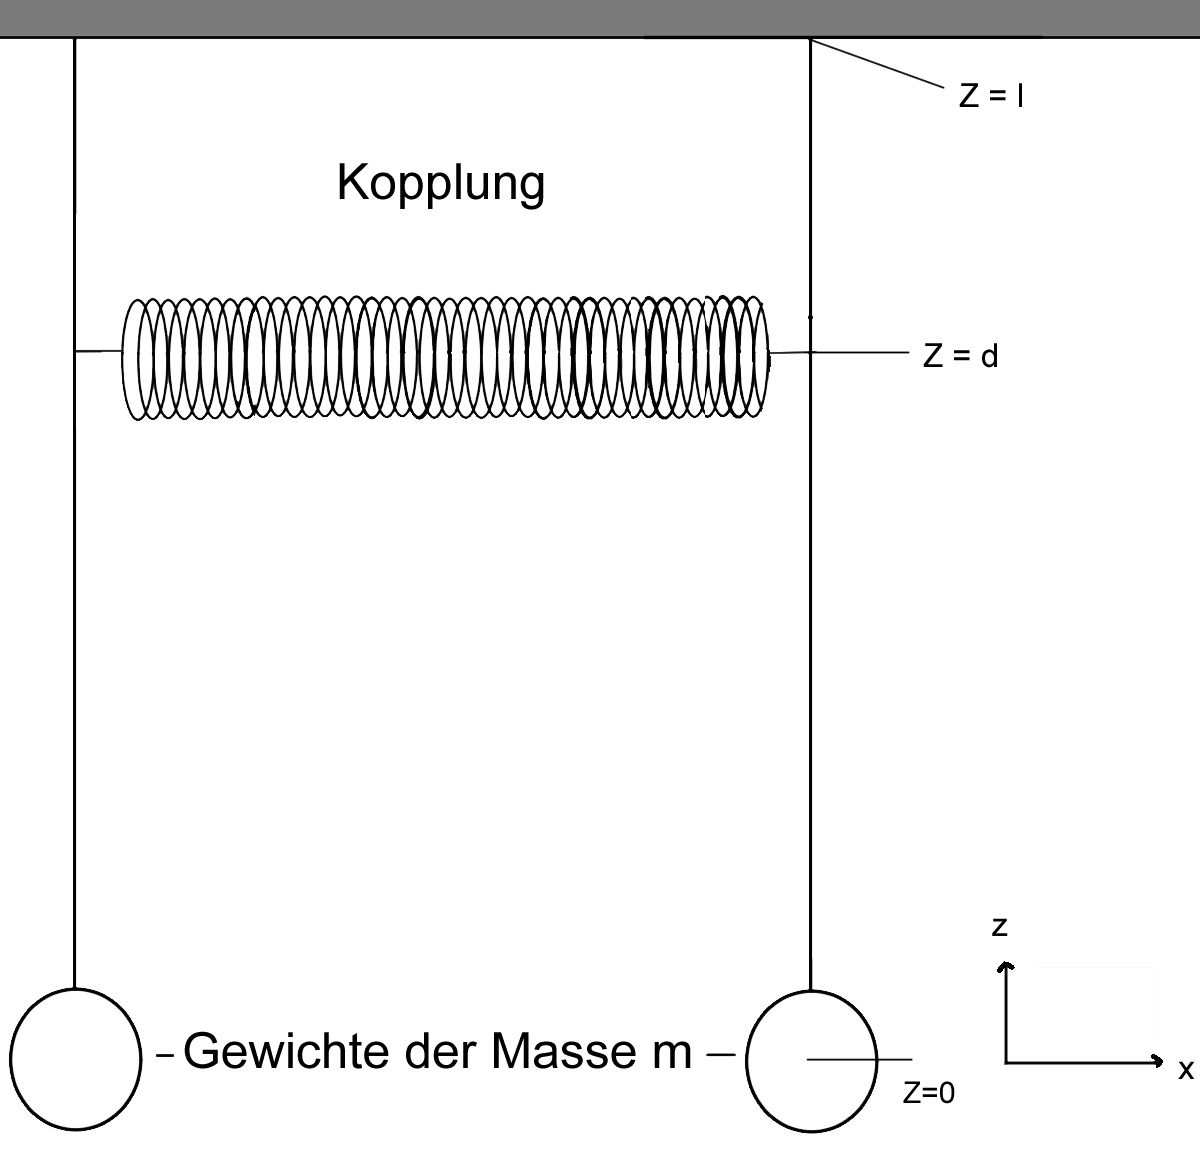
\includegraphics[width=\textwidth]{gFadenpendel.png}
				\caption{gekoppelte Fadenpendel}
				\label{abb:gFadenpendel}	
			\end{figure}
			Hier besitzen beide Pendel die gleiche Länge $l$, hier bei ca. \SI{159}{\cm} (von dem Aufhängepunkt zum Schwerpunkt der Pendel), und Gewichte der Masse $m$. Des Weiteren werden die Fäden für die Berechnung als masselos angenommen. Zur Kopplung der beiden Fadenpendel dienen hierbei zwei verschiedene Federn, welche bei ungefähr $z=d=\SI{113}{\cm}$ zwischen den Pendeln angebracht werden. Bei diesen handelt es sich um eine Kupfer- und um eine Stahlfeder.
			
			Gemessen wird die Auslenkung des Pendels mit Hilfe eines Ultraschall-Entfernungssensors. Diese wird gegen die Zeit aufgetragen, um die Schwingungsdauer $T$ bzw. die Frequenz $\omega$ zu ermitteln. Der Sensor misst mit \SI{50}{\Hz}. Die Messung wird für die Schwingungsdauer ohne Kopplung, für gleich- und gegen-gesinnte Bewegungen sowie für den Fall der Schwebung bei beiden Feder.
			Zudem wird die Auslenkung beider Pendel zur statischen Bestimmung des Kopplungsgrades mit einem Maßband gemessen. 

			Zur Berechnung des Kopplungsgrades wird folgende Formel für den statischen Fall verwendet: 
			\begin{equation}
				k = \frac{x_1}{x_2}. \label{eq:statisch}
			\end{equation}
			Für den dynamischen Fall werden die gemessenen Schwingungsdauern für die gleich- und gegen-gesinnte Bewegung verwendet:
			\begin{align}
				k = \frac{T_\text{gl}^2-T_\text{geg}^2}{T_\text{gl}^2+T_\text{geg}^2}. \label{eq:dynamisch} \\
				\text{bzw. für die Frequenz:} \quad k = \frac{\omega_\text{geg}^2-\omega_\text{gl}^2}{\omega_\text{geg}^2+\omega_\text{gl}^2}.
			\end{align}
			Zuletzt wird die relative Frequenzaufspaltung $\Delta\omega / \omega_0$ mit Hilfe der ermittelten Schwingungsdauern berechnet, dazu:
			\begin{equation}
				\frac{\Delta\omega}{\omega_0} = \frac{\omega_\text{geg}-\omega_\text{gl}}{\omega_\text{gl}} = 2\frac{T_\text{gl}}{T_\text{S}}. \label{eq:freqfrac} 	
			\end{equation}		
			Ebenso lässt sich die Frequenzaufspaltung auch mit der Näherung über die Reihenentwicklung von $\sqrt{1\pm k}$ bis zur 3. Ordnung bestimmen. Mit Umformen von \refeq{dynamisch} und Näherung folgt:
			\begin{equation}
				\frac{\Delta\omega}{\omega_0} = \sqrt\frac{1+k}{1-k}-1 = k + \frac{k^2}{2} + \frac{k^3}{2}. \label{eq:freqfrac2} 
			\end{equation}
		
		\newpage			
		\subsection*{Unsicherheiten}
			
			Die Unsicherheiten wurden wie folgt festgelegt:
			\begin{itemize}
				\item Messgerät: Aus der Messrate von $\SI{50}{\hertz}$ folgt $u_C(T) = \frac{\SI{0,02}{\second}}{2\sqrt{3}}$.
				Zudem ist die Ausgabe der gemessenen Werte auf zwei Nachkommastellen bzw. auf \SI{1}{\cm} genau. Daraus folgt $u_C(x) = \frac{\SI{0,01}{m}}{2\sqrt{3}}$.
				\item Maßband: Von diesem ließ sich mit einer Ungenauigkeit von \SI{0,5}{mm} ablesen. Demnach ist $u(x) = \frac{\SI{0,001}{m}}{2\sqrt{6}}$.
				\item Messung über mehrere Perioden: Der Mittelwert ist gegeben durch $T = \frac{T_j - T_i}{j-i}$.
				Da $T_i$ und $T_j$ jeweils einzelne Messpunkte sind, gilt $u(T_i) = u(T_j) = u(T)$, somit folgt:
				\begin{equation}
					u(T) = \sqrt{\left( \frac{\partial\, T}{\partial\, T_i} u(T)\right)^2 + \left( \frac{\partial\, T}{\partial\, T_j} u(T)\right)^2}
					=\frac{u(T)}{j-i}
				\end{equation}
				\item Schwebung: Da sich das Pendel bei der Schwebung an den Knoten nicht bewegt, ist eine entsprechend große Unsicherheit für einen einzelnen Schwingungsbauch zu wählen (gemäß der Breite des Intervalls der nahezu gleichen Werte).
				Die gemittelte Zeit ist gegeben durch $T_S = 2\frac{T_j - T_i}{j-i}$. Der Faktor $2$ stammt daher, dass eine Periode jeweils zwei Schwingungsbäuche umfasst.
				Mit der Formel für kombinierte Unsicherheiten ergibt sich:
				\begin{equation}
					u(T_S) = \sqrt{\left( \frac{\partial\, T}{\partial\, T_i} u(T_i)\right)^2 + \left( \frac{\partial\, T}{\partial\, T_j} u(T_j)\right)^2}
					=\frac{2}{j-i} \sqrt{u^2(T_i) + u^2(T_j)}.
				\end{equation}
				$T_i$ beschreibt hierbei die Zeit bei dem $i$-ten Knotenpunkt.
			\end{itemize}
			
		\subsection{Messung ohne Kopplung}
										
			Die Messung ergab für den ungekoppelten Fall, dass die Schwingungsdauer $T_0 = \SI{2,4833 +- 0,0001}{\second}$ bzw. die Frequenz $\omega_0 = \SI{0,40269 +- 0,00002}{\s^{-1}}$ entspricht. Hierzu wurden die Differenzen der Nullstellen bei der Messung gebildet und gemittelt. 
			
		\subsection{Messung mit Kupferfeder als Kopplung}
			
			\subsubsection{Statische Ermittlung des Kopplungsgrades}							
				
				Der Kopplungsgrad wird durch Einsetzen in \refeq{statisch} statisch bestimmt. Dies liefert einen Wert von $k=$. Hierfür wurden acht Wertepaare verwendet. Zum Vergleich dient die Abbildung \ref{}.
				
			\subsubsection{Gleich-gesinnte Schwingung}
			
				Für die gleich-gesinnte Bewegung bei der Kupferfeder ergab sich, dass die Schwingungsdauer $T_\text{gl} = \SI{2,4736 +- 0,0001}{\second}$ bzw. die Frequenz $\omega_\text{gl}  = \SI{0,40427 +- 0,00001}{\s^{-1}}$ entspricht. Hierzu wurden die Differenzen der Nullstellen bei der Messung gebildet und gemittelt. 
			
			\subsubsection{Gegen-gesinnte Schwingung}
				
				Bei der gegen-gesinnten Bewegung der Kupferfeder ergab sich, dass die Schwingungsdauer $T_\text{geg} = \SI{2,4157 +- 0,0001}{\second}$ bzw. die Frequenz $\omega_\text{geg}  = \SI{0,41396 +- 0,00002}{\s^{-1}}$ entspricht. Hierzu wurden die Differenzen der Nullstellen bei der Messung gebildet und gemittelt. 
				
			\subsubsection{Schwebung}
				
				Die Messung ergab, dass die Schwingungsdauer $T_\text{S} = \SI{206,03 +-0,68}{\second}$ im Falle der Schwebung entspricht. Da die Periodenzahl bei der Schwebung sehr gering war, wurden für die Bestimmung der Periodendauer die Differenzen der Nullstellen und der Minima gebildet und gemittelt.

			\subsubsection{Relative Frequenzaufspaltung}
				
				Einsetzten in \refeq{freqfrac} liefert eine relative Frequenzaufspaltung von $\Delta\omega / \omega_0 = 0$ über die ermittelten Schwingungsdauern. Über die Näherung aus \refeq{freqfrac2} erhält man hierbei eine Aufspaltung von $\Delta\omega / \omega_0 = 0$.
				
		\subsection{Messung mit Stahlfeder als Kopplung}	
					
			\subsubsection{Statische Ermittlung des Kopplungsgrades}							
			
				Der Kopplungsgrad wird durch Einsetzen in \refeq{statisch} statisch bestimmt. Dies liefert einen Wert von $k=$. Hierfür wurden neun Wertepaare verwendet. Zum Vergleich dient die Abbildung \ref{}.
			
			\subsubsection{Gleich-gesinnte Schwingung}
			
				Für die gleich-gesinnte Bewegung bei der Kupferfeder ergab sich, dass die Schwingungsdauer $T_\text{gl} = \SI{2,4697 +- 0,0001}{\second}$ bzw. die Frequenz $\omega_\text{gl}  = \SI{0,40491 +- 0,00002}{\s^{-1}}$ entspricht. Hierzu wurden die Differenzen der Nullstellen bei der Messung gebildet und gemittelt. 
			
			\subsubsection{Gegen-gesinnte Schwingung}
			
				Bei der gegen-gesinnten Bewegung der Kupferfeder ergab sich, dass die Schwingungsdauer $T_\text{geg} = \SI{2,3753 +- 0,0001}{\second}$ bzw. die Frequenz $\omega_\text{geg}  = \SI{0,42100 +- 0,00002}{\s^{-1}}$ entspricht. Hierzu wurden die Differenzen der Nullstellen bei der Messung gebildet und gemittelt. 
			
			\subsubsection{Schwebung}
			
				Die Messung ergab, dass die Schwingungsdauer $T_\text{S} = \SI{104,52 +- 0,24}{\second}$ im Falle der Schwebung entspricht.  Da die Periodenzahl bei der Schwebung sehr gering war, wurden für die Bestimmung der Periodendauer die Differenzen der Nullstellen und der Minima gebildet und gemittelt.
				% Grafik, Referenz
			
			\subsubsection{Relative Frequenzaufspaltung}
			
				Einsetzten in \refeq{freqfrac} liefert eine relative Frequenzaufspaltung von $\Delta\omega / \omega_0 = 0$ über die ermittelten Schwingungsdauern. Über die Näherung aus \refeq{freqfrac2} erhält man hierbei eine Aufspaltung von $\Delta\omega / \omega_0 = 0$.
																
		\subsection{Ergebnisse und Diskussion}	
			
			\reftab{result} zeigt die Ergebnisse der Messungen für die verschiedenen Kopplungen, damit diese besser verglichen werden können. Hier ist ebenfalls der dynamisch bestimmte Kopplungsgrad aufgelistet, welcher sich durch Einsetzen in \refeq{dynamisch} berechnen ließ, sowie die durch:
			\begin{equation}
				T_\text{S} = \frac{4\pi}{\omega_\text{geg} - \omega_\text{gl}} 
			\end{equation}
			berechneten Schwebungsdauern.
			\begin{table}[ht]
				\caption{Ergebnisse der Versuchsreihe}
				\centering
				\label{tab:result}
				\begin{tabular}{l|S|S}
						& {Methode} & {Ergebnis}\\
					\hline
					{\textbf{ohne Kopplung}} & &\\
					{$T_0$} & {gemessen} & \SI{2,4833 +- 0,0001}{\second}\\
					{$\omega_0$} & {aus $T_0$} & \SI{0,40269 +- 0,00002}{\s^{-1}}\\
					\hline
					{\textbf{Kupferfeder}} & &\\
					{$T_\text{gl}$} & {gemessen} & \SI{2,4736 +- 0,0001}{\second}\\
					{$\omega_\text{gl}$} & {aus $T_\text{gl}$} & \SI{0,40427 +- 0,00001}{\s^{-1}}\\
					{$T_\text{geg}$} & {gemessen} & \SI{2,4157 +- 0,0001}{\second}\\
					{$\omega_\text{geg}$} & {aus $T_\text{geg}$} & \SI{0,41396 +- 0,00002}{\s^{-1}}\\
					{$T_\text{S}$} & {gemessen} & \SI{206,03 +-0,68}{\second}\\
					{$T_\text{S}$} & {berechnet} & \SI{0}{\second}\\
					{$k$} & {statisch} & \SI{0}{\second}\\
					{$k$} & {dynamisch} &\SI{0}{\second}\\
					{$\Delta\omega / \omega_0$} & {berechnet} & \SI{0}{\second}\\
					{$\Delta\omega / \omega_0$} & {genähert} & \SI{0}{\second}\\
					\hline
					{\textbf{Stahlfeder}} & &\\
					{$T_\text{gl}$} & {gemessen} & \SI{2,4697 +- 0,0001}{\second}\\
					{$\omega_\text{gl}$} & {aus $T_\text{gl}$} & \SI{0,40491 +- 0,00002}{\s^{-1}}\\
					{$T_\text{geg}$} & {gemessen} & \SI{2,3753 +- 0,0001}{\second}\\
					{$\omega_\text{geg}$} & {aus $T_\text{geg}$} & \SI{0,42100 +- 0,00002}{\s^{-1}}\\
					{$T_\text{S}$} & {gemessen} & \SI{104,52 +- 0,24}{\second}\\
					{$T_\text{S}$} & {berechnet} & \SI{0}{\second}\\
					{$k$} & {statisch} & \SI{0}{\second}\\
					{$k$} & {dynamisch} & \SI{0}{\second}\\
					{$\Delta\omega / \omega_0$} & {berechnet} & \SI{0}{\second}\\
					{$\Delta\omega / \omega_0$} & {genähert} & \SI{0}{\second}\\
				\end{tabular}
			\end{table}
			%TODO
			Diskussion
		\subsection{Schlussfolgerung}
			
			1 nice Messung				
			%TODO
			
	\section{Doppelpendel}
	
		\subsection{Aufbau und Funktionsweise}	
			
			Das Doppelpendel besteht aus zwei gekoppelten Pendeln. Hierbei ist das obere Pendel an einem festen Aufhängepunkt angebracht. Das Untere  hingegen ist an dem beweglichen Massepunkt des oberen Pendels befestigt. Die Abbildungen \ref{abb:DP_Ruhe}) bis \ref{abb:DP_ausgelenkt}) zeigen die Funktionsweise des Doppelpendels. Hier sind die verschiedenen Auslenkungsmöglichkeiten zu erkennen, wobei die Massepunkte der einzelnen Pendel sich jeweils auf Kreisbahnen um deren Aufhängepunkte bewegen können.	
			\begin{figure}[ht]
				\begin{subfigure}{0.5\textwidth}
					\centering
					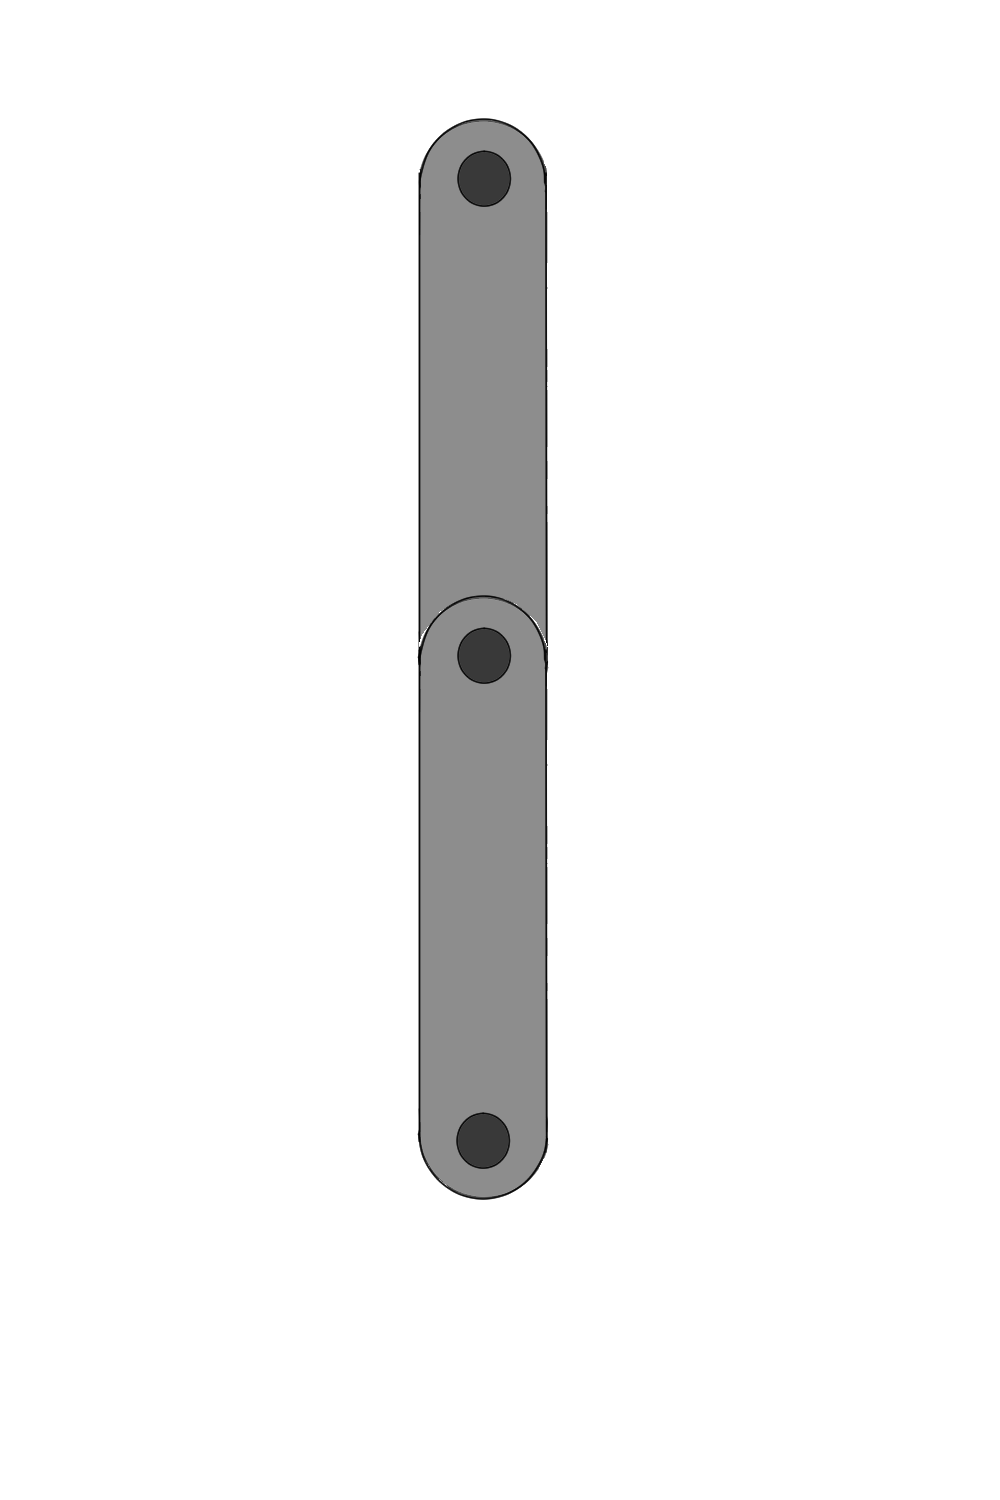
\includegraphics[width=0.5\textwidth]{Doppelpendel_Ruhelage.png}
					\caption{Doppelpendel in Ruhelage}
					\label{abb:DP_Ruhe}	
				\end{subfigure}
				\begin{subfigure}{0.5\textwidth}
					\centering
					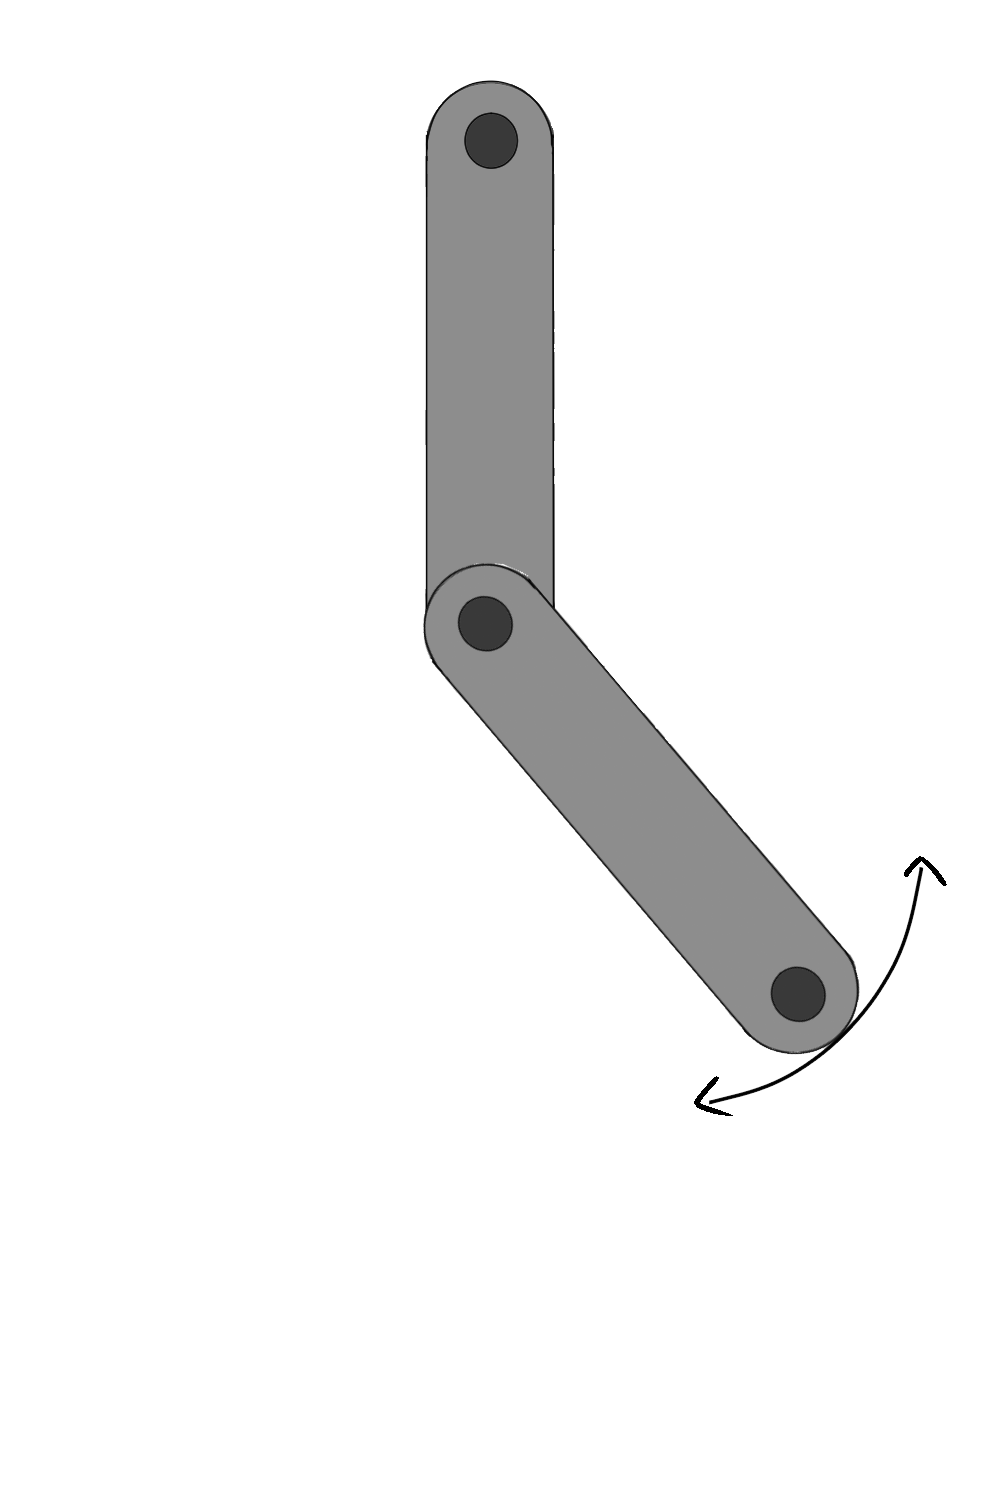
\includegraphics[width=0.5\textwidth]{Doppelpendel_Auslenkung_P2.png}
					\caption{Oberes Pendel in Ruhelage, Unteres ausgelenkt}
					\label{abb:DP_RobenAunten}
				\end{subfigure}
				\begin{subfigure}{0.5\textwidth}
					\centering
					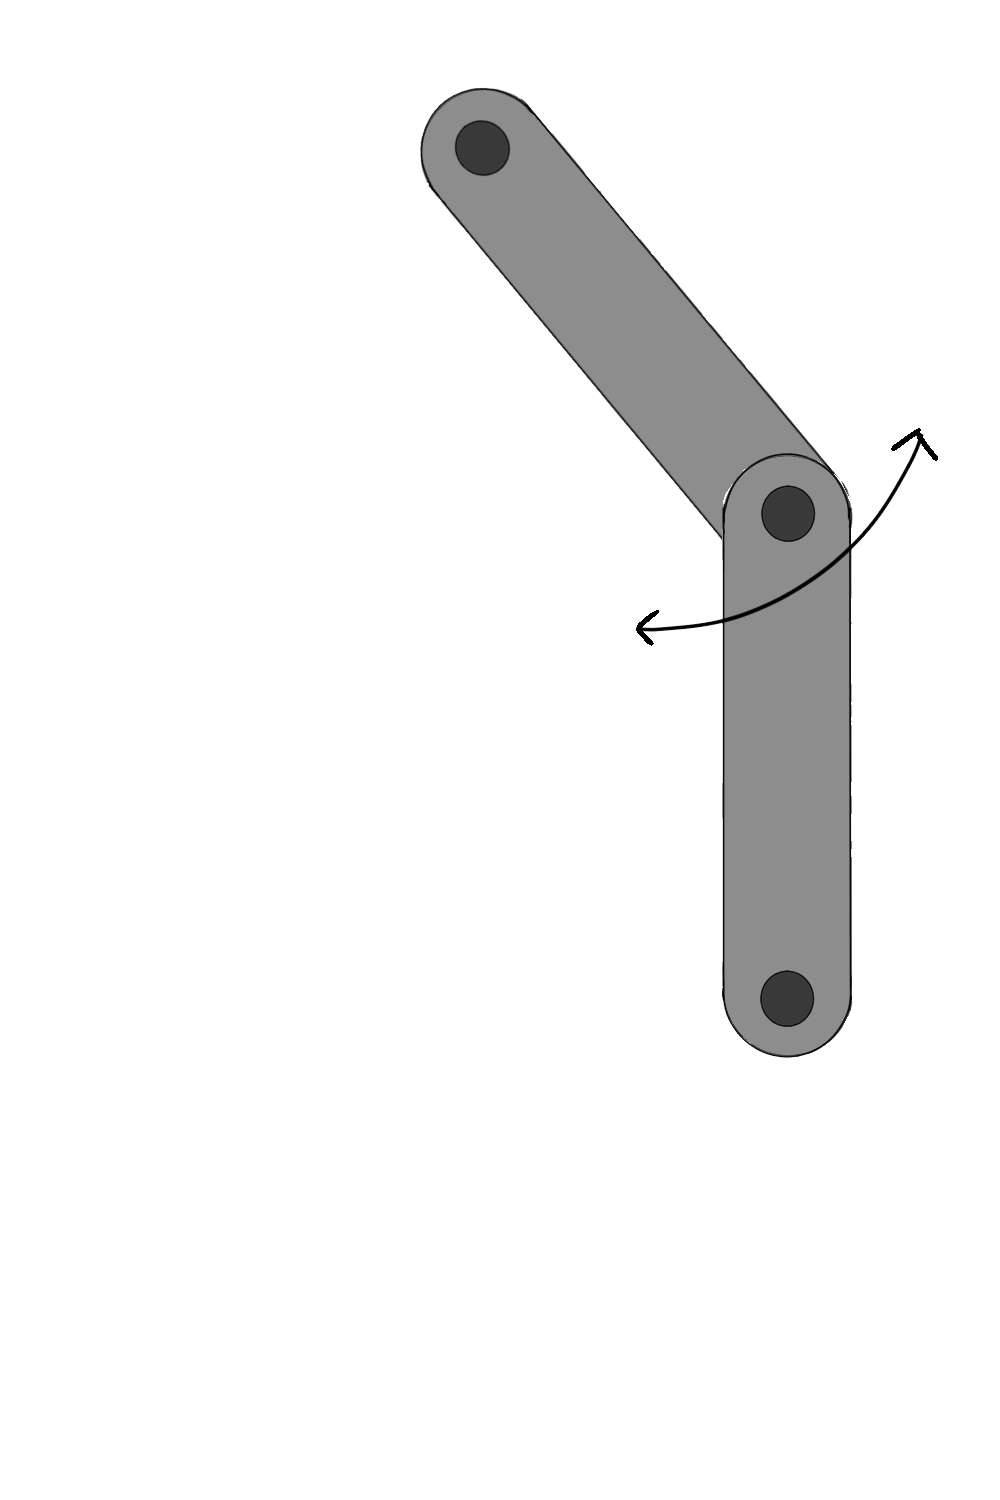
\includegraphics[width=0.5\textwidth]{Doppelpendel_Auslenkung_P1.png}
					\caption{Unteres Pendel in Ruhelage, Oberes ausgelenkt}
					\label{abb:DP_RuntenAoben}
				\end{subfigure}
				\begin{subfigure}{0.5\textwidth}
					\centering
					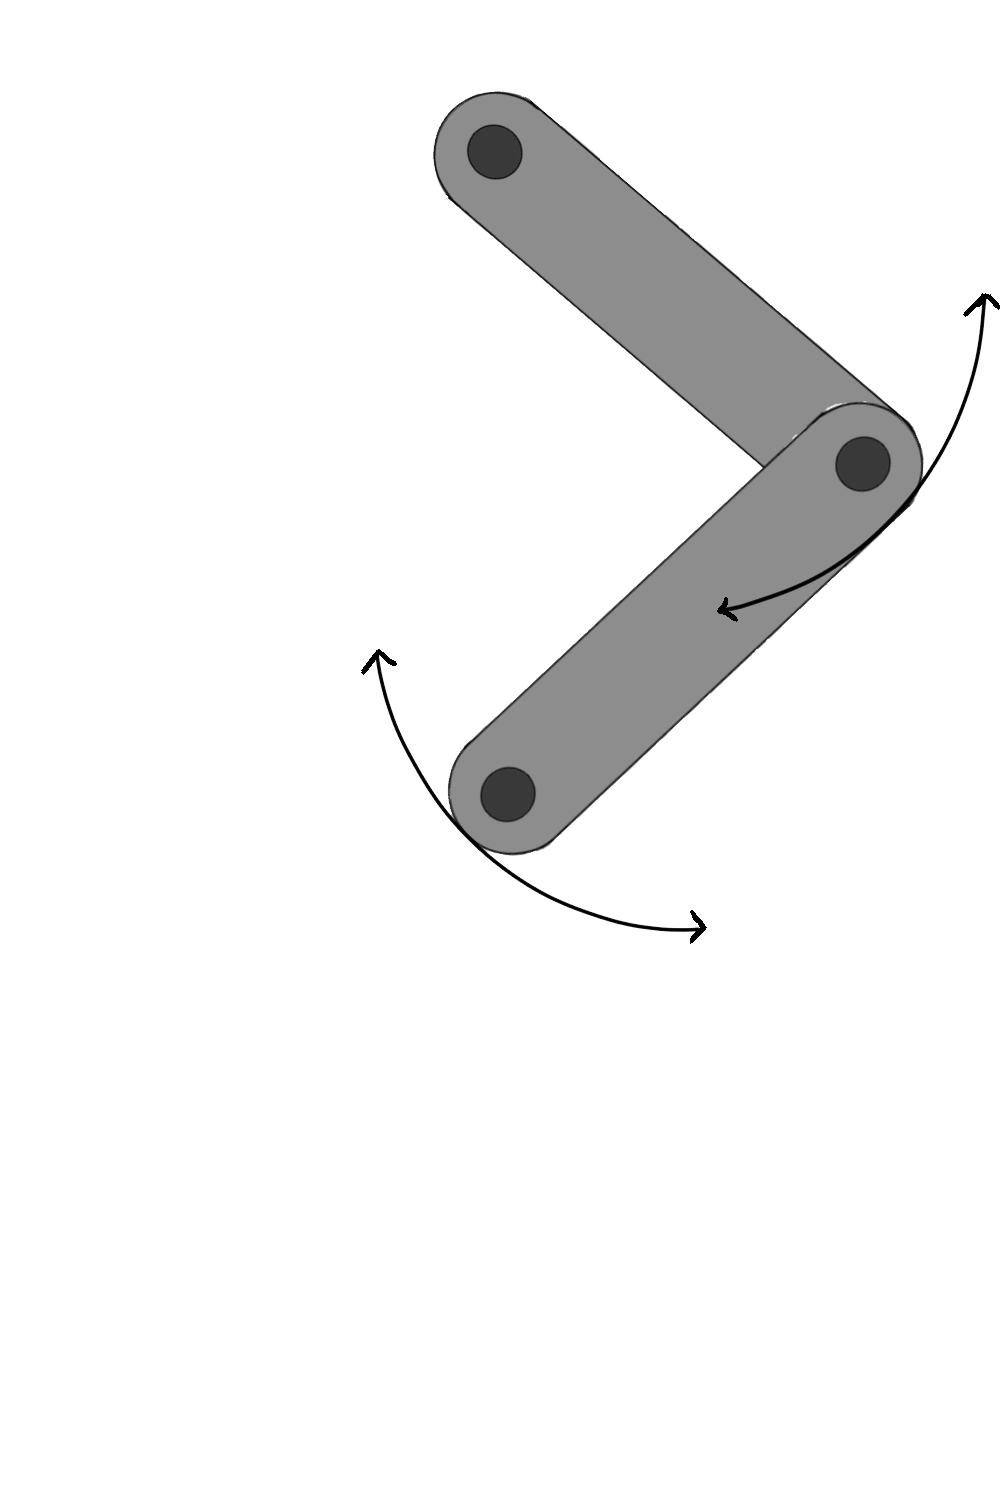
\includegraphics[width=0.5\textwidth]{Doppelpendel_Auslenkung_beide.png}
					\caption{Beide Pendel ausgelenkt}
					\label{abb:DP_ausgelenkt}
				\end{subfigure}		
			\end{figure}
		
		\subsection{Beobachtung bei Auslenkung}
		
			Bei der Auslenkung des Doppelpendels lässt sich ein nichtlineares bzw. chaotisches Verhalten erkennen, da nach nur wenigen Schwingungen, bei nahezu gleichen Anfangsbedingungen, bereits stark unterschiedliche Bewegungen beobachtet wurden. Ein periodisches Verhalten ließ sich hierbei nicht erkennen.
		
			Die Ausnahmen hierzu bilden die Schwingungen, bei Auslenkungen ähnlich zu den, wie sie in \refabb{DP_Ruhe}) und \refabb{DP_ausgelenkt}) dargestellt sind. Bei der ersten linearen Bewegung bewegt sich der Massepunkt des unteren Pendels auf einer Kreisbahn um den Aufhängepunkt des Oberen. Die beiden Pendel liegen bei dieser Bewegung parallel. Für den zweiten Fall einer linearen Bewegung sind die beide Pendel um den gleichen Winkel, jedoch in entgegengesetzte Richtung ausgelenkt, wie es in \refabb{DP_ausgelenkt} dargestellt ist (hier $\pm \ang{45}$). Hier bewegt sich der Massepunkt des unteren Pendels weder nach links noch nach rechts, sondern nur näher dem Aufhängepunkt des oberen Pendels. Dieser Effekt war jedoch nur bei einem Auslenkungswinkel von ca. $\pm \ang{10}$ zu beobachten. Bei größeren Auslenkungen traten erneut nichtlineare Bewegungen auf.
			
			Diese linearen Bewegung ähneln der gleich- bzw. gegen-gesinnten Bewegung der gekoppelten Fadenpendel.  


\end{document} 